% Four observability surfaces over one ground truth for Ch24 ("Observability: Seeing What the Agent Did").
% Standalone TikZ; compiled by `book-scaffold build-figures` via pdflatex -> pdftocairo -> SVG.
% Base: the session log (per-session JSONL transcript) as the single ground truth.
% Above it, four surfaces that DERIVE from it: tracing (OTel GenAI spans/metrics),
% attribution (diff/PR back to the run), cost-surfacing (three altitudes: /usage, team
% dashboard, Console spend), and logging/retention (local 30-day sweep vs SDK SessionStore).
\documentclass[tikz,border=4mm]{standalone}
\usepackage{tikz}
\usetikzlibrary{positioning, arrows.meta, calc}

\begin{document}
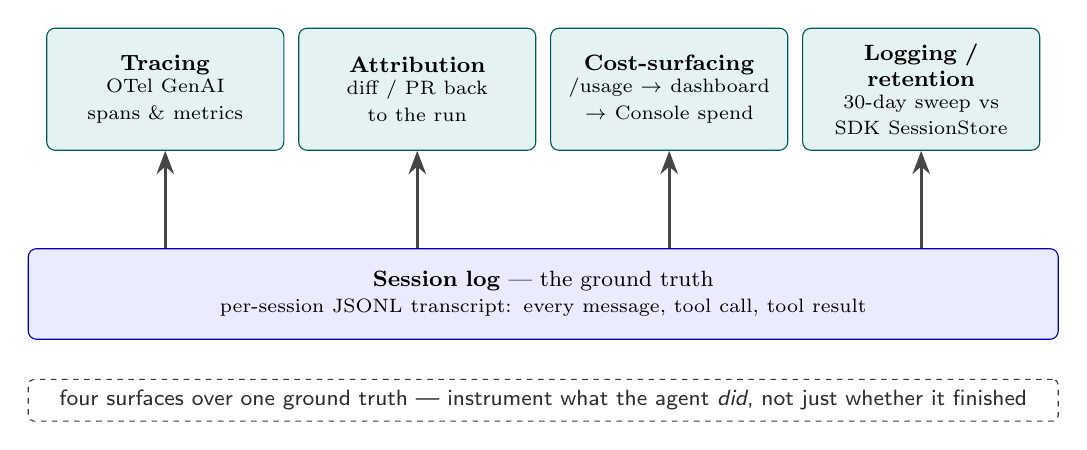
\begin{tikzpicture}[
  font=\sffamily,
  ground/.style={draw=blue!70!black, fill=blue!8, rounded corners=3pt, align=center,
    text width=12.8cm, minimum height=1.15cm, inner sep=4pt, font=\footnotesize},
  surface/.style={draw=teal!70!black, fill=teal!10, rounded corners=3pt, align=center,
    text width=2.8cm, minimum height=1.55cm, inner sep=3pt, font=\footnotesize},
  flow/.style={-Stealth, very thick, draw=gray!55!black},
  note/.style={draw=gray!45!black, dash pattern=on 2pt off 2pt, rounded corners=2pt,
    align=center, inner sep=4pt, font=\sffamily\footnotesize, text=gray!35!black}
]

% --- the single ground truth at the base ---
\node[ground] (log) at (0,0)
  {\textbf{Session log} --- the ground truth\\{\scriptsize per-session JSONL transcript: every message, tool call, tool result}};

% --- four surfaces deriving FROM the log ---
\node[surface] (trace) at (-4.8,2.6)
  {\textbf{Tracing}\\{\scriptsize OTel GenAI\\spans \& metrics}};
\node[surface] (attr) at (-1.6,2.6)
  {\textbf{Attribution}\\{\scriptsize diff / PR back\\to the run}};
\node[surface] (cost) at (1.6,2.6)
  {\textbf{Cost-surfacing}\\{\scriptsize /usage $\rightarrow$ dashboard\\$\rightarrow$ Console spend}};
\node[surface] (ret) at (4.8,2.6)
  {\textbf{Logging /}\\\textbf{retention}\\{\scriptsize 30-day sweep vs\\SDK SessionStore}};

% derive-from arrows: each surface is built on the one log beneath it
\draw[flow] (log.north -| trace.south) -- (trace.south);
\draw[flow] (log.north -| attr.south)  -- (attr.south);
\draw[flow] (log.north -| cost.south)  -- (cost.south);
\draw[flow] (log.north -| ret.south)   -- (ret.south);

% caption strip beneath the ground truth
\node[note, text width=12.8cm] at (0,-1.35)
  {four surfaces over one ground truth --- instrument what the agent \emph{did}, not just whether it finished};

\end{tikzpicture}
\end{document}
